\chapter{Introduction}
\label{chap:intro}

Assume you are in your first year of the Belgium university of Ghent. Like most university students, you live in a dorm and unless you lived in Ghent before moving, you do not know your way in Ghent. You ask yourself what is the best restaurant, what can you do for fun. But at some point you must go to your course, take an exam or take a break from student life at your parent's home. Being late is not option in these situations. But as a first-year and carless, you wonder how you will reach these destinations.  


The most obvious would be \acrfull{pt}. It is a economic way to move yourself through the city without breaking the bank as car would easily cost ten times more on a yearly basis. Further more it is one of the few transportation modes that is environment friendly.

Now you know, how you could reach those destinations. You question which route is best to take. Further, you want to be sure if you will arrive on time and at which time you should leave. 

For this last problem, there is a high chance that you will use a route planner. Many route planners exist, like \url{nmbs.be}, \url{delijn.be} or \url{maps.google.com}. Even open-source solutions exist like Open Trip Planner\cite{raptorinopentripplanner}.

Underlying these route planners, an algorithm calculates the "best" route serving your search criteria. They produce pareto-optimal journeys. A journey is defined as a sequence of trips between two points. A trip can be made using a variety of vechicles (train, bus,...) or even by foot. One thing to remark is that if a journey contains $K$ trips, then they are $K-1$ transfers. % TODO FINSIH THIS EXPLANATION + TO MUCH DETAIL IN INTRODUCTION ???j

Commonly, these algorithms are graph-based. Although known speedup techniques can achieve speedups of up to several million on route planners, these speedups are generally more focused on road networks \cite{raptor}. When looking at a more specific domain, like \acrshort{pt}. A few difficulties arise.

% difficulties road planners and PT
To start, \acrshort{pt} has a different structure than for road networks. For example, the travel times are enough as criteria to compute a road journey, but for \acrshort{pt}, additional criteria could be the number of transfers or the cost of the diffrent transportation modes (train, bus, metro,...). These extra criteria adds more complexity to the calculations.

Footpaths are a significant influence on the resulting Pareto journeys. It could be more efficient to walk to a different bus stop. But, unrestricted footpaths would cause too many edges in graph-based algorithms.

Most route planners use a centralized data strategy. \cite{julianIntro}
\begin{enumerate}
    \item Collect, for each transit mode, a dataset. A widely used format for exchanging a PT dataset is GTFS \cite{GTFS}.
    \item Integrate the collected datasets using a predefined data model in a centralized data store.
    \item Calculates available routes using a route planning algorithm tailored to run over the predefined data model.
\end{enumerate}
% Our focus

This thesis's main focus is on removing the centralized data strategy;

The centralized strategy causes applications to be unscalable and results in high costs of computational infrastructure (total cost of ownership). 

% work in progress
Another problem is that if a third-party dataset is not supported by the central system, the user can not use the dataset in his queries. The data needs to be homogenous to be able to integrate it into the route planner. If the dataset is heterogeneous, then integration is done manually and the route planner algorithm has to be adapted.
\section{Goal}

\begin{figure}[H]
\centering
\resizebox{\textwidth}{!}{
\begin{tikzpicture}

\draw [stealth-stealth](0,0) -- (10,0);

\draw (10,0) node[above=32pt,right=-2.5 cm] {2013: Connection Scan Algorithm};

\end{tikzpicture}}
    \caption{This figure represents what we want to accomplish a solution that not only runs on the client and not only on the server.}
    \label{fig:shared}
\end{figure}


\begin{figure}[H]
    \centering
    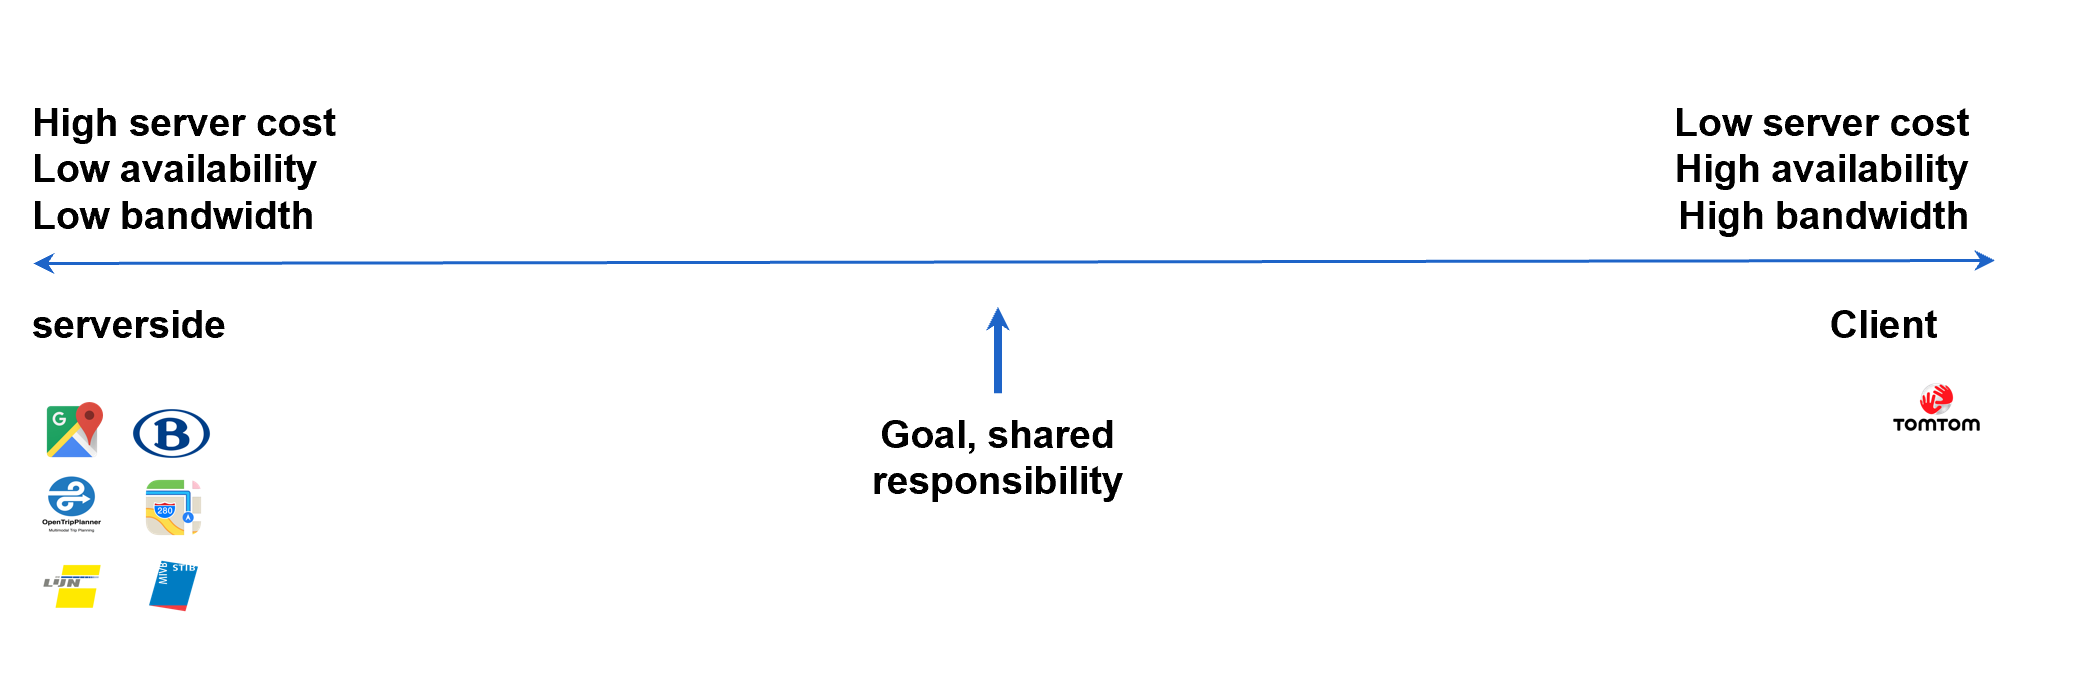
\includegraphics[width=\textwidth]{images/shared responsibility.PNG}
    \caption{}
    \label{fig:sharedresponsibility}
\end{figure}
\section{Introduction to important concepts}
\subsection{Semantic Web}
The semantic web is a vision of Tim Berners-Lee, where web documents not only describe how to render data visually. The data is also annotated with terms to express how it should be interpreted. So web documents also capture the meaning of the information.

\subsection{Ontologies: what \& why}
The best definition of an ontology states: "An ontology is an explicit specification of a conceptualization"\cite{GRUBER1993199}. Many ontologies exist, from basic to formal ontologies specified in highly expressive logic. In this thesis, we mainly use formal ontologies.

These ontologies play an essential role in the semantic web. 